%\chapter{Vorlesung}


\chapter{Verallgemeinerung von Akra-Bazzi}
\label{ch:12}

\[T_n = \left[\sum_{i=1}^k a_i T(\frac{n}{b_i}) \right] + g(n) \]
\paragraph{Beispiel}
\[T_n = 1\cdot T\left(\frac{n}{3}\right)+1\cdot T\left(\frac{2n}{3}\right) + n \]
\[T_n = \theta\left(n^{\alpha}\left(1+\int_1^n\frac{g\left(x\right)}{x^{1+\alpha}} dx\right)\right)  \]


\paragraph{Klassisch} $\alpha = \log_b(a)$, $\frac{a}{b^{\alpha}} = 1$
\paragraph{Jetzt} Bestimmte $\alpha$ so, dass gilt:
\[\sum_{i=1}^k \frac{a_i}{b_i^{\alpha}} = 1 \]
\[a_1 = a_2 = 1, ~~~~ b_1 = 3, ~~~~ b_2 = \frac{3}{2}, ~~~~ g(n) = n \]
 \[\frac{1}{3}^{\alpha} + \frac{2}{3}^{\alpha} \overset{!}{=} 1 \Rightarrow \alpha = 1 \]
\[T(n) = \Theta \left(n \left(1+\int_1^n \frac{x}{x^{1+1}} dx\right) \right) = \Theta(n\ln(n)) \]


\chapter{Median der Mediane}
\section{Ansatz} %Ergänzung von Markus
\subsubsection*{Gruppierung in 5er Päckchen}
\begin{wrapfigure}[7]{l}{0.4\linewidth}
\vspace{-40pt}
\centering
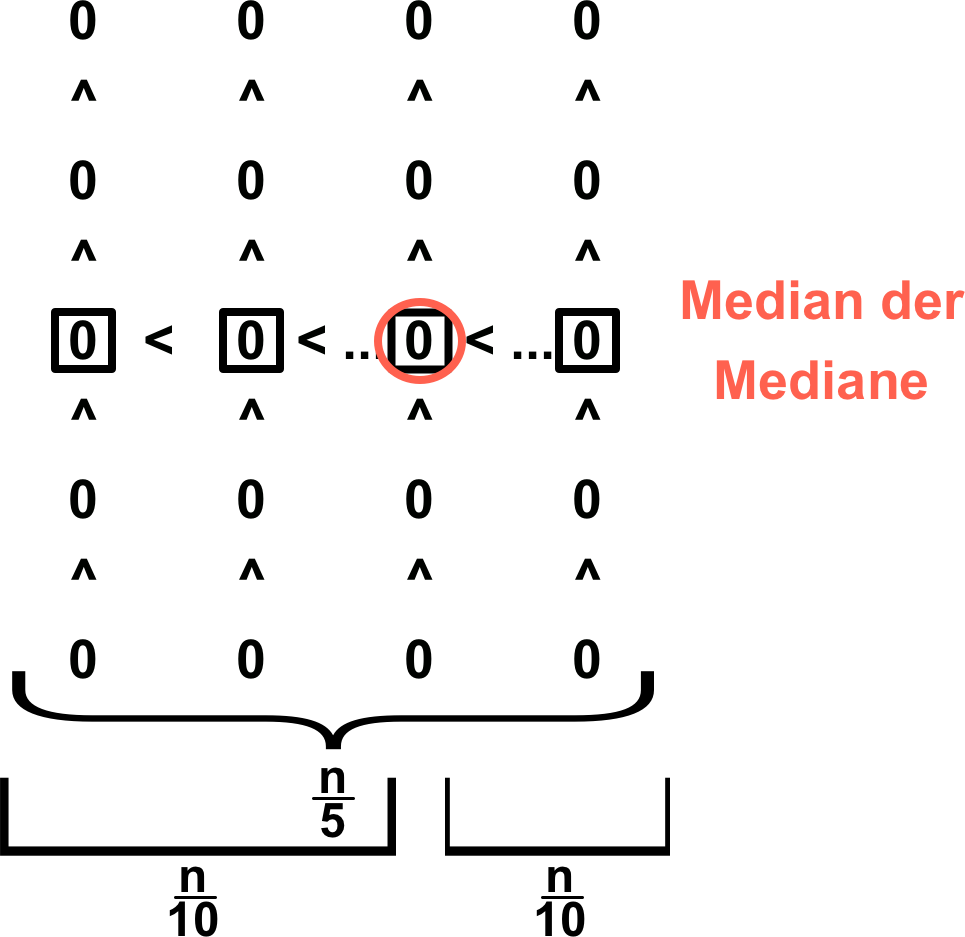
\includegraphics[width=0.6\linewidth]{08/Grafik/img1.png}
\caption{Median der Mediane}
\end{wrapfigure}

\vspace{20pt}
\paragraph{Wortlaut}
Teile die n Elemente in 5-er Gruppen. Bestimme innerhalb jeder Gruppe den Median. Bestimme nun den Median der Mediane. Wähle diesen Median als Pivotelement.
\[\exists \frac{3n}{10}~\text{Elemente}~\leq p \geq \exists \frac{3n}{10}~\text{Elemente}~(\pm 1~\text{wegen p})\]
\vspace{1pt}


%\newpage


\section{Deterministische Variante für k-Select}
Wähle zu Beginn den Median der Mediane als Pivot Elemente. Unterteile nun die Folge anhand von $p$ in zwei Teilfolgen und verfahre von nun an analog zur randomisierten Variante von k-Select.

\section{Laufzeitanalyse für den worst-case}
\[T(n) = T\left(\frac{n}{5}\right)+n+T \left(\frac{7n}{10} \right) \]
\[A_1 = \frac{n}{5},~~~~A_2 = n,~~~~A_3= \frac{7n}{10}\]
$A_1$ = Laufzeit zur rekursiven Bestimmung des Medians der Mediane mittels k-Select\\
$A_2$ = Laufzeit zur Aufteilung in Teilfolgen\\
$A_3$ = Laufzeit für den Aufruf von k-Select  für die größere Teilfolge in jedem Durchlauf, die aber sicher $\leq n - \frac{3n}{10} = \frac{7n}{10}$ hat.\\

Wende die verallgemeinerte Form von Akra-Bazzi an:\\
$g(n)=n, ~~~a_1=a_2=1, ~~~b_1=5, ~~~b_2=\frac{10}{7}$\\
\paragraph{Bestimme}
\[\alpha = \left(\frac{1}{5}\right)^{\alpha} + \left(\frac{7}{10}\right)^{\alpha} = 1\]
\[\Leftrightarrow \left(\frac{2}{10}\right)^{\alpha} + \left(\frac{7}{10}\right)^{\alpha} = 1\]
\[\Rightarrow 0 < \alpha < 1 \]
	\[\textstyle\centering n^{\alpha}\left(1+\int_1^n \frac{x}{x^{1+\alpha}} dx\right) = n^{\alpha}\left(1+\int_1^n x^{-\alpha} dx\right) = n^{\alpha}\left(1+ \left[\frac{1}{1-\alpha} x^{-\alpha+1} \right]_1^n\right) = n^{\alpha}\left(1+\frac{1}{1-\alpha} \left(n^{-\alpha+1}-1\right)\right)\]

%\newpage

\chapter{Untere Schranke für vergleichsbasierte Sortierverfahren}
\section{Entscheidungsproblem: (Bubbelsort)}
\begin{figure}[h]
	\centering
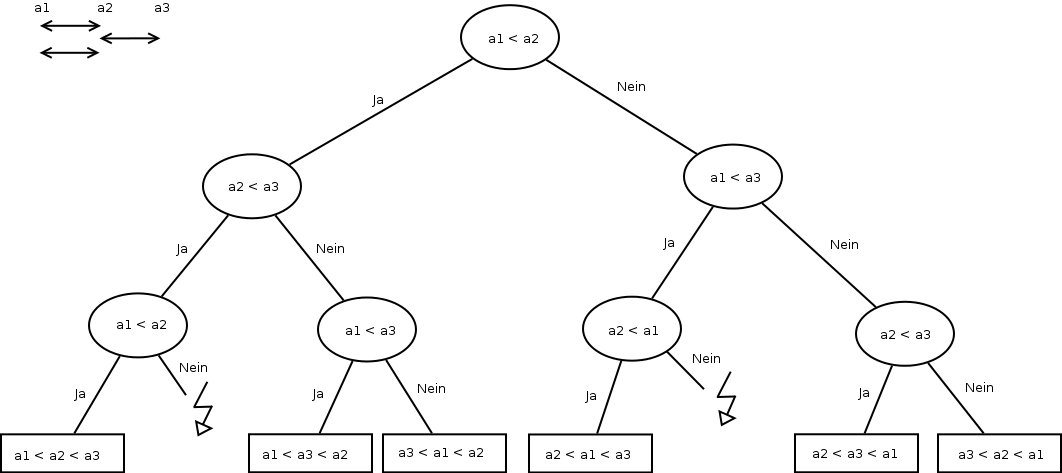
\includegraphics[width=\linewidth]{08/Grafik/img2.png}
\caption{Entscheidungsbaum am Beispiel Bubblesort}
\end{figure}


Ein Entscheidungsbaum für einen vergleichsbasierten Sortieralgorithmus besteht aus inneren Knoten, die mit der Vergleichsoperation $a_i < a_j$ beschriftet sind, wobei sich die Indizes $i,j$ auf die Position der Elemente in der Eingabefolge beziehen.\\
Die Blätter des Entscheidungsbaums sind mit den Permutationen beschriftet, die sich nach korrekter Sortierung ergeben.\\
Jeder korrekte Sortieralgorithmus muss zu einem Entscheidungsbaum mit mindestens $n!$ Blättern korrespondieren.\\
\paragraph{maximale Baumtiefe} $~\hat{=}~$ maximale Anzahl durchgeführter Vergleichsoperationen\\
\paragraph{mittlere Baumtiefe} $~\hat{=}~$ average-case Laufzeit
